%%%%%%%%% Notes %%%%%%%%%

%%%%%%%%% Packages %%%%%%%%%
\documentclass[aspectratio=43]{beamer}
\usepackage[T1]{fontenc}
\usepackage{derivative}
\usepackage{pgfpages}

%%%%%%%%% Packages setup %%%%%%%%%
\setbeameroption{show notes on second screen}
%\setbeameroption{show only notes}
%\setbeamerfont{note page}{size=\tiny}
\setbeamercolor{note page}{bg=white, fg=black}
\setbeamercolor{note title}{bg=white!99!black, fg=black}
\usetheme{Hannover}
\usecolortheme{spruce}
\graphicspath{{./figures/}{../code/figures/}}

%%%%%%%%% Document informations %%%%%%%%%
\title{Summary of \emph{A tutorial on the free-energy framework for modelling perception and learning} by Rafal Bogacz}
\author{Marco Casari}
\date[12/12/2023]{Complex system in neuroscience, 12 December 2023}
\institute[UniTo]{University of Turin}

%%%%%%%%% Document %%%%%%%%%
\begin{document}
\begin{frame}
  \titlepage
  \note{
    \begin{itemize}
      \item % MC general overview of presentation.
    \end{itemize}
  }
\end{frame}



\section{Introduction}
\begin{frame}
  \frametitle{Introduction}
  \begin{itemize}
    \item<1-> Predictive coding model of Rao and Ballard.
    \note[item]<1->{Prior predictions are compared to stimuli and the model parameters are updated considering prediction errors, features corresponding to receptive fields in the the primary sensory cortex are learned.}
    \item<2-> Free-energy model of Friston.
    \note[item]<2->{Weight stimuli by their noise, learn features using their covariance, implement attentional modulation changing the variance of attended features.}
    \item<3-> Hebbian plasticity.
    \note[item]<3->{Synaptic strenght is changed proportionally to activities of pre-synaptic and post-synaptic neurons.}
    \item<4-> Free energy minimization.
    \note[item]<4->{Minimization of free energy can be seen as the base of many theories of perception.}
  \end{itemize}
\end{frame}

\begin{frame}
  \frametitle{Working hypotheses}
  \begin{itemize}
    \item<1-> Local computation.
    \note[item]<1->{The state of a neuron is determined only by the synaptic weight and the state of its input neurons.}
    \item<2-> Local plasticity.
    \note[item]<2->{Synaptic plasticity depends only on the activities of pre-synaptic and post-synaptic neurons.}
    \item<3-> Basic neuronal computation.
    \note[item]<3->{The state of a neuron is the result of the application of a monotonic function to the linear combination of states and synaptic weights of input neurons.}
  \end{itemize}
\end{frame}



\section{Single variable model}
\begin{frame}
  \frametitle{Single variable model}
  \begin{itemize}
    \item<1-> Feature is a scalar variable $v \in \Omega_v$.
    \item<1-> Stimulus is a scalar variable $u \in \Omega_u$.
    \note[item]<1->{The model describes the inference of a single variable from a single sensory input.}
    \item<2-> Relation between feature and stimulus is a differentiable function $g : \Omega_v \to \Omega_u$.
    \note[item]<2->{In general inferred variable and sensory input are related by some smooth function.}
    \item<3-> Sensory input $p(u|v)$ is affected by gaussian noise and it has mean $g(v)$ and variance $\Sigma_u$.
    \note[item]<3->{Sensory input and stimulus are drafted from the same space.}
    \item<4-> Prior knowledge of the feature $p(v)$ follows a gaussian distribution with mean $v_p$ and variance $\Sigma_p$.
    \note[item]<4->{Information gained and constantly updated from previous experience.}
  \end{itemize}
\end{frame}

\begin{frame}
  \frametitle{Exact solution of the inference problem}
  \begin{itemize}
    \item<1-> Bayes theorem:
      \begin{equation}
        \label{eq:bayes}
        p(v|u) = \frac{p(v) p(u|v)}{p(u)}
        \quad .
      \end{equation}
    \note[item]<1->{Knowledge of feature depending on a given stimulus is the posterior. Prior knowledge on the feature is the prior, distribution of stimulus is the likelihood.}
    \item<2-> Marginal likelihood of stimuli:
      \begin{equation}
        \label{eq:marginal}
        p(u) = \int_{\Omega_v} p(v) p(u|v) \odif{v}
        \quad .
      \end{equation}
    \note[item]<2->{In general, marginal likelihood is difficult to evaluate.}
    \item<3-> No implementation in simple biological systems.
    \note[item]<3->{Complex calculations and infinite nodes are needed to represent each value of the posterior.}
  \end{itemize}
\end{frame}

% MC insert Exercise_1.

\begin{frame}
  \frametitle{Approximated solution of the inference problem}
  \begin{itemize}
    \item<1-> Most likely value of the feature is a scalar variable $\phi \in \Omega_v$.
    \note[item]<1->{Evaluating the mode of the posterior instead of the whole function is more biologically plausible.}
    \item<2-> Equivalent to minimize negative free energy:
      \begin{equation}
        \label{eq:negative_free_energy}
        F(v, u) = \ln{\big( p(v) \big)} + \ln{\big( p(u|v) \big)}
        \quad .
      \end{equation}
    \note[item]<2->{The most likely feature value is the fixed point of the gradient descent method applied to the negative free energy.}
    \item<3-> Prediction errors:
      \begin{align}
        \label{eq:error_prior}
        \epsilon_p = \frac{v - v_p}{\Sigma_p}
        \quad , \\
        \label{eq:error_stimulus}
        \epsilon_u = \frac{u - g(v)}{\Sigma_u}
        \quad .
      \end{align}
    \note[item]<3->{Prediction errors can be introduced as new variables to extend the dynamical system.}
  \end{itemize}
\end{frame}

% MC insert Exercise_2.

\begin{frame}
  \frametitle{Neural implementation}
  \begin{center}
    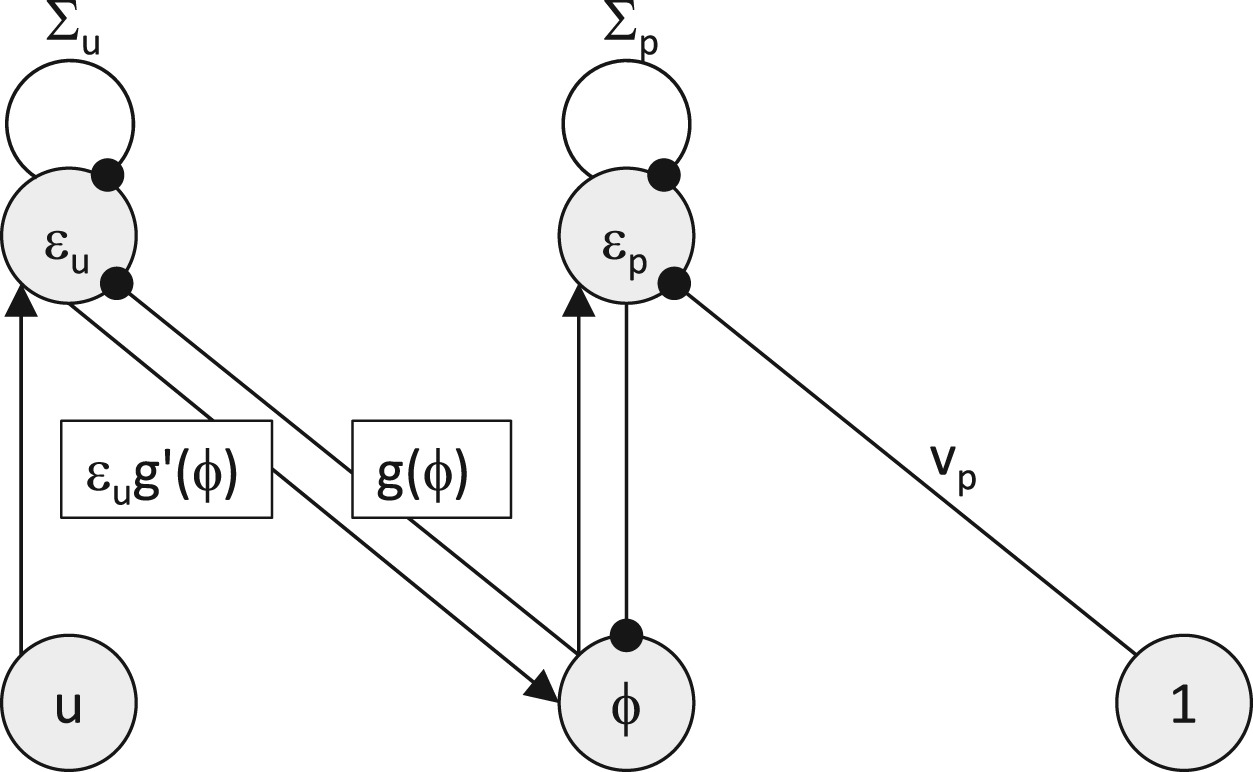
\includegraphics[width=0.5\textheight]{Fig3}
  \end{center}
  Fig. 3 from article: network implementation of the dynamical system
  \begin{equation}
    \label{eq:dynamical_system_single}
    \begin{cases}
      \dot{\phi} = \epsilon_u g^\prime(\phi) - \epsilon_p \\
      \dot{\epsilon_p} = \phi - v_p - \Sigma_p \epsilon_p \\
      \dot{\epsilon_u} = u - g(\phi) - \Sigma_u \epsilon_u
    \end{cases}
    \quad .
  \end{equation}
  \note{
    \begin{itemize}
      \item Hypotheses on local computation and Hebbian plasticity are satisfied.
    \end{itemize}
  }
\end{frame}

% MC insert Exercise_3.

% MC here talk about prediction errors.
\begin{frame}
  \frametitle{Learning model parameters}
  \begin{itemize}
    \item<1-> % MC continue.
    \note[item]<1->{Introducing prediction errors as variables of the model allows to learn model parameters.}
  \end{itemize}
\end{frame}

\begin{frame}
  \frametitle{Learning relation between variable and stimulus}
  \begin{itemize}
    \item % MC continue.
  \end{itemize}
\end{frame}

\begin{frame}
  \frametitle{Free energy framework}
  \begin{itemize}
    \item % MC continue.
  \end{itemize}
\end{frame}



% MC here hint to the use of matrix algebra.
\section{Multiple variables model}
\begin{frame}
  \frametitle{Multiple variables model}
  \begin{itemize}
    \item % MC continue.
  \end{itemize}
\end{frame}

% MC here talk about prediction errors.
\begin{frame}
  \frametitle{Learning parameters}
  \begin{itemize}
    \item % MC continue.
  \end{itemize}
\end{frame}

\begin{frame}
  \frametitle{Hierarchical structure implementation}
  \begin{itemize}
    \item % MC continue.
  \end{itemize}
\end{frame}

% MC here just hint to the possibility of extending local plasticity to mutliple layers (cf. 5.2).
\begin{frame}
  \frametitle{Recover local plasticity}
  \begin{itemize}
    \item % MC continue.
  \end{itemize}
\end{frame}

% MC insert Exercise_5.



% MC here resume the Discussion.
\section{Conclusion}
\begin{frame}
  \frametitle{Conclusion}
  \begin{itemize}
    \item % MC complete with resume of content and future work.
  \end{itemize}
%  \vfill
%  \onslide<2->{
%    \centering
%    \huge
%    Thank you
%  }
\end{frame}
\end{document}
